\newif\ifsolutions
\solutionstrue % Show solutions
%\solutionsfalse % Hide solutions

\documentclass{article}
\usepackage{geometry}
\geometry{margin=1in}
\usepackage{tikz}
\usepackage{amssymb}

% fleqn allows setting indent of display math
\usepackage[fleqn]{amsmath}
\setlength{\mathindent}{0pt} % Set indent
% Disable equation numbering (https://tex.stackexchange.com/a/360378)
\makeatletter
\renewcommand\tagform@[1]{}
\makeatother

% Allow Unicode (some, e.g., © and £ at least)
% https://tex.stackexchange.com/questions/370278/is-there-any-reason-to-use-inputenc
\usepackage[utf8]{inputenc}

% Hyperlinks
\usepackage{hyperref}
\hypersetup{colorlinks=true, urlcolor=blue, linkcolor=blue}

% Prevent indentation of paragraphs
\setlength\parindent{0pt}
\setlength{\parskip}{\baselineskip}

% Spacing above/below equations
% https://tex.stackexchange.com/a/69678
\AtBeginDocument{%
 \abovedisplayskip=-\parskip
 \abovedisplayshortskip=-\parskip
 \belowdisplayskip=0pt
 \belowdisplayshortskip=0pt
}

% Allow 3 additional subsection levels
% https://tex.stackexchange.com/a/60212
\usepackage{titlesec}
\setcounter{secnumdepth}{6}
% H4 in HTML
\titleformat{\paragraph}{\normalfont\normalsize\bfseries}{\theparagraph}{1em}{}
\titlespacing*{\paragraph}{0pt}{3.25ex plus 1ex minus .2ex}{1.5ex plus .2ex}
% H5 in HTML
\titleformat{\subparagraph}{\normalfont\normalsize\bfseries}{\thesubparagraph}{1em}{}
\titlespacing*{\subparagraph}{0pt}{3.25ex plus 1ex minus .2ex}{1.5ex plus .2ex}
% H6 in HTML
\titleformat{\subsubparagraph}{\normalfont\normalsize\bfseries}{\thesubsubparagraph}{1em}{}
\titlespacing*{\subsubparagraph}{0pt}{3.25ex plus 1ex minus .2ex}{1.5ex plus .2ex}

% So enumerate at all levels is numbers
% https://tex.stackexchange.com/questions/78842/nested-enumeration-numbering
\renewcommand{\labelenumii}{\arabic{enumii}.}
\renewcommand{\labelenumiii}{\arabic{enumiii}.}
\renewcommand{\labelenumiv}{\arabic{enumiv}.}

\renewcommand{\mbox}{\text}
\newcommand{\ds}[0]{\displaystyle}
\newcommand{\ihat}[0]{\hat{\boldsymbol{\imath}}}
\newcommand{\jhat}[0]{\hat{\boldsymbol{\jmath}}}
\newcommand{\khat}[0]{\hat{\boldsymbol{k}}}
\newcommand{\xhat}[0]{\hat{\mathbf{x}}}
\newcommand{\yhat}[0]{\hat{\mathbf{y}}}
\newcommand{\zhat}[0]{\hat{\mathbf{z}}}
\newcommand{\rhat}[0]{\hat{\mathbf{r}}}
\newcommand{\bfvec}[1]{\vec{\mathbf{#1}}}
\newcommand{\bfcdot}[0]{\boldsymbol{\cdot}}

\usepackage{fancyhdr}
\pagestyle{fancy}
\lhead{Electric Force}
\rhead{\thepage}
\fancyfoot{}

\begin{document}

% Figures:
% https://www.mathcha.io/editor/M55KMuQLiLmH9Vgp0Ptw6QGB3HnpzJnnuM6VoB7

\section{Coulomb's Law}

\emph{Magnitude}

$$F_{1\mbox{ on } 2}=F_{2\mbox{ on } 1}=k\frac{|q_1q_2|}{r^2}$$

where $r$ is the distance between $q_1$ and $q_2$. To simplify notation, we are using $k$ in place of $1/4\pi\epsilon_o$. Note that by definition, the magnitude of a vector is positive, which is the reason for the use of the absolute value.

\emph{Direction}: Along line that connects $q_1$ and $q_2$. Direction depends on signs of $q_1$ and $q_2$. (Likes repel, opposites attract.).

\section{Example}

Charge $q_1$ is at $(x,y)=(-a,-a)$ and charge $q_2$ is at $(a, a)$. Both charges have a charge of $q$.

\begin{enumerate}

  \item Find the magnitude of the force of $q_1$ on $q_2$.

  \item Find the direction of the force of $q_1$ on $q_2$ in terms of an angle with respect to the $+x$--axis with counterclockwise positive.

  \item Write the force of $q_1$ on $q_2$ in the form $\bfvec{F}=F_x\ihat + F_y\jhat$.

  \item If $q_1=q$ and $q_2=-q$, how will your answers to 1.--3. change?

  \item If $q_1=-q$ and $q_2=-q$, how will your answers to 1.--3. change?

\end{enumerate}

\textbf{Solution}

\begin{enumerate}

  \item The distance between the charges is $r=\sqrt{(2a)^2+(2a)^2}=\sqrt{8a^2}$, so

        $$F_{1\mbox{ on } 2}=k\frac{|q_1q_2|}{r^2}=\frac{k|qq|}{(\sqrt{8a^2})^2}=\frac{kq^2}{8a^2}$$

  \item The charges will repel each other, so the direction of forces of one on the other will be as shown in the left part of the following diagram. The angle of $F_{1\mbox{ on } 2}$ is $+45^\circ$ with respect to the $+x$--axis with counterclockwise positive.

        

\tikzset{every picture/.style={line width=0.75pt}} %set default line width to 0.75pt        

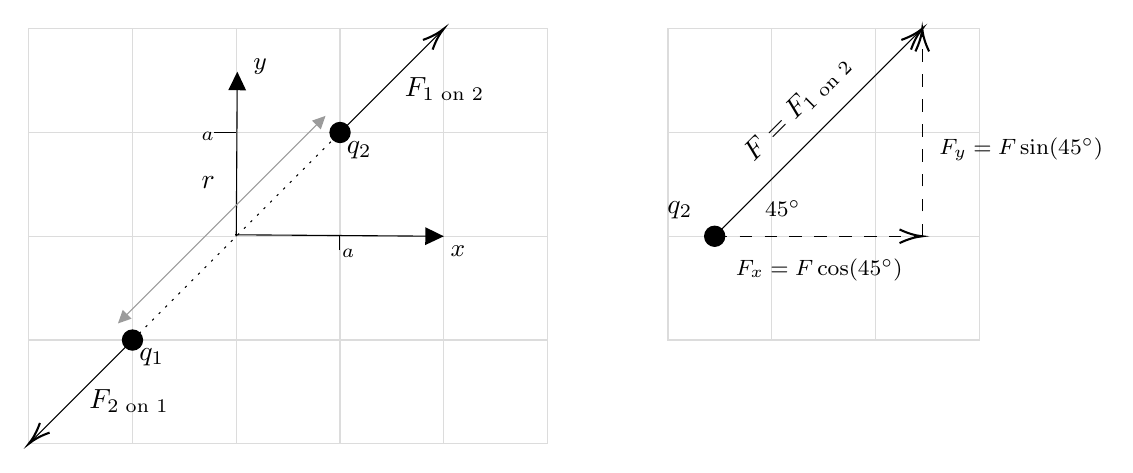
\begin{tikzpicture}[x=0.75pt,y=0.75pt,yscale=-1,xscale=1]
%uncomment if require: \path (0,244); %set diagram left start at 0, and has height of 244

%Shape: Grid [id:dp19152925292042688] 
\draw  [draw opacity=0] (330.5,12) -- (480.5,12) -- (480.5,162) -- (330.5,162) -- cycle ; \draw  [color={rgb, 255:red, 220; green, 220; blue, 220 }  ,draw opacity=1 ] (380.5,12) -- (380.5,162)(430.5,12) -- (430.5,162) ; \draw  [color={rgb, 255:red, 220; green, 220; blue, 220 }  ,draw opacity=1 ] (330.5,62) -- (480.5,62)(330.5,112) -- (480.5,112) ; \draw  [color={rgb, 255:red, 220; green, 220; blue, 220 }  ,draw opacity=1 ] (330.5,12) -- (480.5,12) -- (480.5,162) -- (330.5,162) -- cycle ;
%Shape: Grid [id:dp21314532969559075] 
\draw  [draw opacity=0] (22.5,12) -- (272.5,12) -- (272.5,212) -- (22.5,212) -- cycle ; \draw  [color={rgb, 255:red, 220; green, 220; blue, 220 }  ,draw opacity=1 ] (72.5,12) -- (72.5,212)(122.5,12) -- (122.5,212)(172.5,12) -- (172.5,212)(222.5,12) -- (222.5,212) ; \draw  [color={rgb, 255:red, 220; green, 220; blue, 220 }  ,draw opacity=1 ] (22.5,62) -- (272.5,62)(22.5,112) -- (272.5,112)(22.5,162) -- (272.5,162) ; \draw  [color={rgb, 255:red, 220; green, 220; blue, 220 }  ,draw opacity=1 ] (22.5,12) -- (272.5,12) -- (272.5,212) -- (22.5,212) -- cycle ;
%Straight Lines [id:da9729239052224414] 
\draw    (122.5,112) -- (122.98,35.71) ;
\draw [shift={(123,32.71)}, rotate = 90.36] [fill={rgb, 255:red, 0; green, 0; blue, 0 }  ][line width=0.08]  [draw opacity=0] (8.93,-4.29) -- (0,0) -- (8.93,4.29) -- cycle    ;
%Straight Lines [id:da4475195096201732] 
\draw    (122,111.29) -- (219.5,111.98) ;
\draw [shift={(222.5,112)}, rotate = 180.41] [fill={rgb, 255:red, 0; green, 0; blue, 0 }  ][line width=0.08]  [draw opacity=0] (8.93,-4.29) -- (0,0) -- (8.93,4.29) -- cycle    ;
%Shape: Circle [id:dp45842230266548145] 
\draw  [fill={rgb, 255:red, 0; green, 0; blue, 0 }  ,fill opacity=1 ] (67.63,162) .. controls (67.63,159.31) and (69.81,157.13) .. (72.5,157.13) .. controls (75.19,157.13) and (77.37,159.31) .. (77.37,162) .. controls (77.37,164.69) and (75.19,166.87) .. (72.5,166.87) .. controls (69.81,166.87) and (67.63,164.69) .. (67.63,162) -- cycle ;
%Straight Lines [id:da7138524881820565] 
\draw    (172.5,62) -- (221.09,13.41) ;
\draw [shift={(222.5,12)}, rotate = 135] [color={rgb, 255:red, 0; green, 0; blue, 0 }  ][line width=0.75]    (10.93,-3.29) .. controls (6.95,-1.4) and (3.31,-0.3) .. (0,0) .. controls (3.31,0.3) and (6.95,1.4) .. (10.93,3.29)   ;
%Shape: Circle [id:dp05463728965143022] 
\draw  [fill={rgb, 255:red, 0; green, 0; blue, 0 }  ,fill opacity=1 ] (167.63,62) .. controls (167.63,59.31) and (169.81,57.13) .. (172.5,57.13) .. controls (175.19,57.13) and (177.37,59.31) .. (177.37,62) .. controls (177.37,64.69) and (175.19,66.87) .. (172.5,66.87) .. controls (169.81,66.87) and (167.63,64.69) .. (167.63,62) -- cycle ;
%Straight Lines [id:da6513912815179692] 
\draw  [dash pattern={on 4.5pt off 4.5pt}]  (353,112) -- (451,112) ;
\draw [shift={(453,112)}, rotate = 180] [color={rgb, 255:red, 0; green, 0; blue, 0 }  ][line width=0.75]    (10.93,-3.29) .. controls (6.95,-1.4) and (3.31,-0.3) .. (0,0) .. controls (3.31,0.3) and (6.95,1.4) .. (10.93,3.29)   ;
%Straight Lines [id:da22911090478458496] 
\draw  [dash pattern={on 4.5pt off 4.5pt}]  (453,112) -- (453,14) ;
\draw [shift={(453,12)}, rotate = 90] [color={rgb, 255:red, 0; green, 0; blue, 0 }  ][line width=0.75]    (10.93,-3.29) .. controls (6.95,-1.4) and (3.31,-0.3) .. (0,0) .. controls (3.31,0.3) and (6.95,1.4) .. (10.93,3.29)   ;
%Straight Lines [id:da09885207354950065] 
\draw    (172.25,118.64) -- (172.25,111.64) ;
%Straight Lines [id:da9341519147192137] 
\draw    (112,62) -- (122.5,62) ;
%Straight Lines [id:da3669669514491145] 
\draw  [dash pattern={on 0.84pt off 2.51pt}]  (72.5,162) -- (172.5,62) ;
%Straight Lines [id:da12376617626287523] 
\draw [color={rgb, 255:red, 155; green, 155; blue, 155 }  ,draw opacity=1 ]   (67.62,151.88) -- (163.38,56.12) ;
\draw [shift={(165.5,54)}, rotate = 135] [fill={rgb, 255:red, 155; green, 155; blue, 155 }  ,fill opacity=1 ][line width=0.08]  [draw opacity=0] (6.25,-3) -- (0,0) -- (6.25,3) -- cycle    ;
\draw [shift={(65.5,154)}, rotate = 315] [fill={rgb, 255:red, 155; green, 155; blue, 155 }  ,fill opacity=1 ][line width=0.08]  [draw opacity=0] (6.25,-3) -- (0,0) -- (6.25,3) -- cycle    ;
%Straight Lines [id:da9907727050490871] 
\draw    (72.5,162) -- (23.91,210.59) ;
\draw [shift={(22.5,212)}, rotate = 315] [color={rgb, 255:red, 0; green, 0; blue, 0 }  ][line width=0.75]    (10.93,-3.29) .. controls (6.95,-1.4) and (3.31,-0.3) .. (0,0) .. controls (3.31,0.3) and (6.95,1.4) .. (10.93,3.29)   ;
%Straight Lines [id:da4068492692003185] 
\draw    (353,112) -- (451.59,13.41) ;
\draw [shift={(453,12)}, rotate = 135] [color={rgb, 255:red, 0; green, 0; blue, 0 }  ][line width=0.75]    (10.93,-3.29) .. controls (6.95,-1.4) and (3.31,-0.3) .. (0,0) .. controls (3.31,0.3) and (6.95,1.4) .. (10.93,3.29)   ;
%Shape: Circle [id:dp7850957636365832] 
\draw  [fill={rgb, 255:red, 0; green, 0; blue, 0 }  ,fill opacity=1 ] (348.13,112) .. controls (348.13,109.31) and (350.31,107.13) .. (353,107.13) .. controls (355.69,107.13) and (357.87,109.31) .. (357.87,112) .. controls (357.87,114.69) and (355.69,116.87) .. (353,116.87) .. controls (350.31,116.87) and (348.13,114.69) .. (348.13,112) -- cycle ;

% Text Node
\draw (129.5,25.4) node [anchor=north west][inner sep=0.75pt]  [font=\small]  {$y$};
% Text Node
\draw (224.5,115.4) node [anchor=north west][inner sep=0.75pt]  [font=\small]  {$x$};
% Text Node
\draw (202.5,34.4) node [anchor=north west][inner sep=0.75pt]    {$F_{\text{1 on 2}}$};
% Text Node
\draw (174.5,65) node [anchor=north west][inner sep=0.75pt]   [align=left] {$\displaystyle q_{2}$};
% Text Node
\draw (376,93.4) node [anchor=north west][inner sep=0.75pt]  [font=\footnotesize]  {$45^{\circ }$};
% Text Node
\draw (362,121.4) node [anchor=north west][inner sep=0.75pt]  [font=\footnotesize]  {$F_{x} =F\cos (45^{\circ } )$};
% Text Node
\draw (460,63.4) node [anchor=north west][inner sep=0.75pt]  [font=\footnotesize]  {$F_{y} =F\sin (45^{\circ } )$};
% Text Node
\draw (172.25,117.04) node [anchor=north west][inner sep=0.75pt]  [font=\scriptsize]  {$a$};
% Text Node
\draw (104.5,60.4) node [anchor=north west][inner sep=0.75pt]  [font=\scriptsize]  {$a$};
% Text Node
\draw (104.5,82) node [anchor=north west][inner sep=0.75pt]   [align=left] {$\displaystyle r$};
% Text Node
\draw (50.5,184.4) node [anchor=north west][inner sep=0.75pt]    {$F_{\text{2 on 1}}$};
% Text Node
\draw (74.5,165) node [anchor=north west][inner sep=0.75pt]   [align=left] {$\displaystyle q_{1}$};
% Text Node
\draw (363.61,69.95) node [anchor=north west][inner sep=0.75pt]  [rotate=-315]  {$F=F_{\text{1 on 2}}$};
% Text Node
\draw (329,94) node [anchor=north west][inner sep=0.75pt]   [align=left] {$\displaystyle q_{2}$};


\end{tikzpicture}


  \item Let $F = F_{1\mbox{ on } 2}$ from part 1. to simplify notation. The right part of the above diagram shows the calculation of the components $F_x$ and $F_y$, from which it follows that $\bfvec{F} = F\cos 45^\circ \ihat + F\sin 45^\circ \jhat$.

  \item 

        p1

        The magnitude will not change (it is by definition a positive number).

        p2

        The force vectors will reverse direction as shown on the left in the following diagram. The angle of $F_{1\mbox{ on } 2}$ is $225^\circ$ with respect to the $+x$ axis with counterclockwise positive.

        p3.

        When the angle $\theta$ of a vector $\bfvec{V}$ is given with respect to $+x$--axis, it can be written in component form without using a diagram using the formula $\bfvec{V} = V\cos\theta\ihat + V\sin\theta\jhat$. Thus,

        $\bfvec{F}_{1\mbox{ on } 2} = F\cos 225^\circ \ihat + F\sin 225^\circ \jhat$.

        Alternatively, the diagram on the right of the following figure shows the calculation of $\bfvec{F}_{1\mbox{ on } 2}$ using a different angle and manually inserting the signs of the components based on the diagram. The result is

        $\bfvec{F}_{1\mbox{ on } 2} = -F\cos 45^\circ \ihat - F\sin 45^\circ \jhat$.

        These two answers are identical (what trig identity can be used to show this?).

        Comparing $\bfvec{F}_{1\mbox{ on } 2} = -F\cos 45^\circ \ihat - F\sin 45^\circ \jhat$ with the answer for part 3. of the original problem, we see that to reverse the direction of a vector, we can multiply each of its components by $-1$.

        

\tikzset{every picture/.style={line width=0.75pt}} %set default line width to 0.75pt        

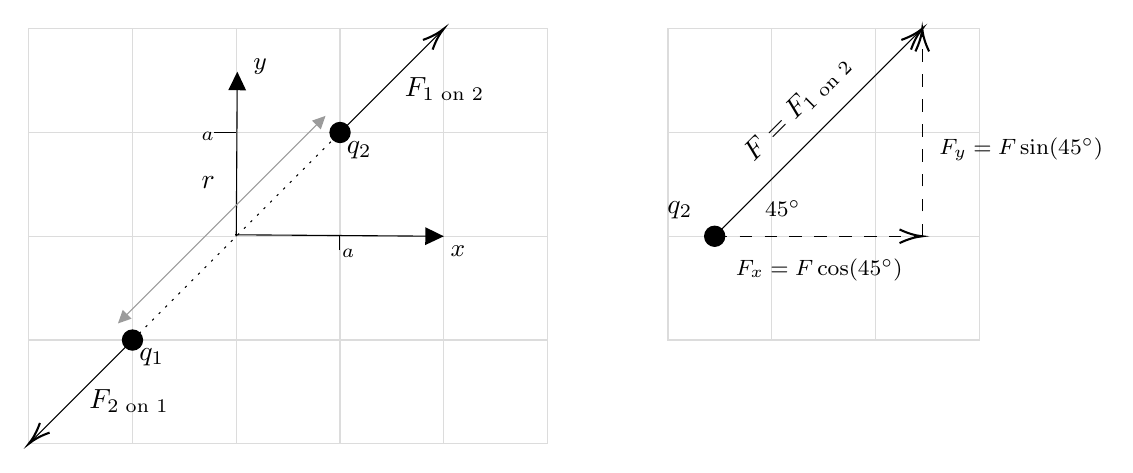
\begin{tikzpicture}[x=0.75pt,y=0.75pt,yscale=-1,xscale=1]
%uncomment if require: \path (0,244); %set diagram left start at 0, and has height of 244

%Shape: Grid [id:dp19152925292042688] 
\draw  [draw opacity=0] (330.5,12) -- (480.5,12) -- (480.5,162) -- (330.5,162) -- cycle ; \draw  [color={rgb, 255:red, 220; green, 220; blue, 220 }  ,draw opacity=1 ] (380.5,12) -- (380.5,162)(430.5,12) -- (430.5,162) ; \draw  [color={rgb, 255:red, 220; green, 220; blue, 220 }  ,draw opacity=1 ] (330.5,62) -- (480.5,62)(330.5,112) -- (480.5,112) ; \draw  [color={rgb, 255:red, 220; green, 220; blue, 220 }  ,draw opacity=1 ] (330.5,12) -- (480.5,12) -- (480.5,162) -- (330.5,162) -- cycle ;
%Shape: Grid [id:dp21314532969559075] 
\draw  [draw opacity=0] (22.5,12) -- (272.5,12) -- (272.5,212) -- (22.5,212) -- cycle ; \draw  [color={rgb, 255:red, 220; green, 220; blue, 220 }  ,draw opacity=1 ] (72.5,12) -- (72.5,212)(122.5,12) -- (122.5,212)(172.5,12) -- (172.5,212)(222.5,12) -- (222.5,212) ; \draw  [color={rgb, 255:red, 220; green, 220; blue, 220 }  ,draw opacity=1 ] (22.5,62) -- (272.5,62)(22.5,112) -- (272.5,112)(22.5,162) -- (272.5,162) ; \draw  [color={rgb, 255:red, 220; green, 220; blue, 220 }  ,draw opacity=1 ] (22.5,12) -- (272.5,12) -- (272.5,212) -- (22.5,212) -- cycle ;
%Straight Lines [id:da9729239052224414] 
\draw    (122.5,112) -- (122.98,35.71) ;
\draw [shift={(123,32.71)}, rotate = 90.36] [fill={rgb, 255:red, 0; green, 0; blue, 0 }  ][line width=0.08]  [draw opacity=0] (8.93,-4.29) -- (0,0) -- (8.93,4.29) -- cycle    ;
%Straight Lines [id:da4475195096201732] 
\draw    (122,111.29) -- (219.5,111.98) ;
\draw [shift={(222.5,112)}, rotate = 180.41] [fill={rgb, 255:red, 0; green, 0; blue, 0 }  ][line width=0.08]  [draw opacity=0] (8.93,-4.29) -- (0,0) -- (8.93,4.29) -- cycle    ;
%Shape: Circle [id:dp45842230266548145] 
\draw  [fill={rgb, 255:red, 0; green, 0; blue, 0 }  ,fill opacity=1 ] (67.63,162) .. controls (67.63,159.31) and (69.81,157.13) .. (72.5,157.13) .. controls (75.19,157.13) and (77.37,159.31) .. (77.37,162) .. controls (77.37,164.69) and (75.19,166.87) .. (72.5,166.87) .. controls (69.81,166.87) and (67.63,164.69) .. (67.63,162) -- cycle ;
%Straight Lines [id:da7138524881820565] 
\draw    (172.5,62) -- (221.09,13.41) ;
\draw [shift={(222.5,12)}, rotate = 135] [color={rgb, 255:red, 0; green, 0; blue, 0 }  ][line width=0.75]    (10.93,-3.29) .. controls (6.95,-1.4) and (3.31,-0.3) .. (0,0) .. controls (3.31,0.3) and (6.95,1.4) .. (10.93,3.29)   ;
%Shape: Circle [id:dp05463728965143022] 
\draw  [fill={rgb, 255:red, 0; green, 0; blue, 0 }  ,fill opacity=1 ] (167.63,62) .. controls (167.63,59.31) and (169.81,57.13) .. (172.5,57.13) .. controls (175.19,57.13) and (177.37,59.31) .. (177.37,62) .. controls (177.37,64.69) and (175.19,66.87) .. (172.5,66.87) .. controls (169.81,66.87) and (167.63,64.69) .. (167.63,62) -- cycle ;
%Straight Lines [id:da6513912815179692] 
\draw  [dash pattern={on 4.5pt off 4.5pt}]  (353,112) -- (451,112) ;
\draw [shift={(453,112)}, rotate = 180] [color={rgb, 255:red, 0; green, 0; blue, 0 }  ][line width=0.75]    (10.93,-3.29) .. controls (6.95,-1.4) and (3.31,-0.3) .. (0,0) .. controls (3.31,0.3) and (6.95,1.4) .. (10.93,3.29)   ;
%Straight Lines [id:da22911090478458496] 
\draw  [dash pattern={on 4.5pt off 4.5pt}]  (453,112) -- (453,14) ;
\draw [shift={(453,12)}, rotate = 90] [color={rgb, 255:red, 0; green, 0; blue, 0 }  ][line width=0.75]    (10.93,-3.29) .. controls (6.95,-1.4) and (3.31,-0.3) .. (0,0) .. controls (3.31,0.3) and (6.95,1.4) .. (10.93,3.29)   ;
%Straight Lines [id:da09885207354950065] 
\draw    (172.25,118.64) -- (172.25,111.64) ;
%Straight Lines [id:da9341519147192137] 
\draw    (112,62) -- (122.5,62) ;
%Straight Lines [id:da3669669514491145] 
\draw  [dash pattern={on 0.84pt off 2.51pt}]  (72.5,162) -- (172.5,62) ;
%Straight Lines [id:da12376617626287523] 
\draw [color={rgb, 255:red, 155; green, 155; blue, 155 }  ,draw opacity=1 ]   (67.62,151.88) -- (163.38,56.12) ;
\draw [shift={(165.5,54)}, rotate = 135] [fill={rgb, 255:red, 155; green, 155; blue, 155 }  ,fill opacity=1 ][line width=0.08]  [draw opacity=0] (6.25,-3) -- (0,0) -- (6.25,3) -- cycle    ;
\draw [shift={(65.5,154)}, rotate = 315] [fill={rgb, 255:red, 155; green, 155; blue, 155 }  ,fill opacity=1 ][line width=0.08]  [draw opacity=0] (6.25,-3) -- (0,0) -- (6.25,3) -- cycle    ;
%Straight Lines [id:da9907727050490871] 
\draw    (72.5,162) -- (23.91,210.59) ;
\draw [shift={(22.5,212)}, rotate = 315] [color={rgb, 255:red, 0; green, 0; blue, 0 }  ][line width=0.75]    (10.93,-3.29) .. controls (6.95,-1.4) and (3.31,-0.3) .. (0,0) .. controls (3.31,0.3) and (6.95,1.4) .. (10.93,3.29)   ;
%Straight Lines [id:da4068492692003185] 
\draw    (353,112) -- (451.59,13.41) ;
\draw [shift={(453,12)}, rotate = 135] [color={rgb, 255:red, 0; green, 0; blue, 0 }  ][line width=0.75]    (10.93,-3.29) .. controls (6.95,-1.4) and (3.31,-0.3) .. (0,0) .. controls (3.31,0.3) and (6.95,1.4) .. (10.93,3.29)   ;
%Shape: Circle [id:dp7850957636365832] 
\draw  [fill={rgb, 255:red, 0; green, 0; blue, 0 }  ,fill opacity=1 ] (348.13,112) .. controls (348.13,109.31) and (350.31,107.13) .. (353,107.13) .. controls (355.69,107.13) and (357.87,109.31) .. (357.87,112) .. controls (357.87,114.69) and (355.69,116.87) .. (353,116.87) .. controls (350.31,116.87) and (348.13,114.69) .. (348.13,112) -- cycle ;

% Text Node
\draw (129.5,25.4) node [anchor=north west][inner sep=0.75pt]  [font=\small]  {$y$};
% Text Node
\draw (224.5,115.4) node [anchor=north west][inner sep=0.75pt]  [font=\small]  {$x$};
% Text Node
\draw (202.5,34.4) node [anchor=north west][inner sep=0.75pt]    {$F_{\text{1 on 2}}$};
% Text Node
\draw (174.5,65) node [anchor=north west][inner sep=0.75pt]   [align=left] {$\displaystyle q_{2}$};
% Text Node
\draw (376,93.4) node [anchor=north west][inner sep=0.75pt]  [font=\footnotesize]  {$45^{\circ }$};
% Text Node
\draw (362,121.4) node [anchor=north west][inner sep=0.75pt]  [font=\footnotesize]  {$F_{x} =F\cos (45^{\circ } )$};
% Text Node
\draw (460,63.4) node [anchor=north west][inner sep=0.75pt]  [font=\footnotesize]  {$F_{y} =F\sin (45^{\circ } )$};
% Text Node
\draw (172.25,117.04) node [anchor=north west][inner sep=0.75pt]  [font=\scriptsize]  {$a$};
% Text Node
\draw (104.5,60.4) node [anchor=north west][inner sep=0.75pt]  [font=\scriptsize]  {$a$};
% Text Node
\draw (104.5,82) node [anchor=north west][inner sep=0.75pt]   [align=left] {$\displaystyle r$};
% Text Node
\draw (50.5,184.4) node [anchor=north west][inner sep=0.75pt]    {$F_{\text{2 on 1}}$};
% Text Node
\draw (74.5,165) node [anchor=north west][inner sep=0.75pt]   [align=left] {$\displaystyle q_{1}$};
% Text Node
\draw (363.61,69.95) node [anchor=north west][inner sep=0.75pt]  [rotate=-315]  {$F=F_{\text{1 on 2}}$};
% Text Node
\draw (329,94) node [anchor=north west][inner sep=0.75pt]   [align=left] {$\displaystyle q_{2}$};


\end{tikzpicture}


  \item The magnitude is the same, as before. The charges repel, so the direction is the same as in the answer to 2. and the force vector is the same as the answer to 3.

        \ifsolutions
        \newpage
        \fi

\end{enumerate}

\section{Problem I}

Charge $q_1$ is at $(x,y)=(-a,a)$ and charge $q_2$ is at $(a, -a)$. Both charges have a charge of $q$. Draw this charge configuration and then using the steps in the previous example,

\begin{enumerate}

  \item Find the magnitude of the force of $q_1$ on $q_2$.

  \item Find the direction of the force of $q_1$ on $q_2$ in terms of an angle with respect to the $+x$--axis with counterclockwise positive.

  \item Write the force of $q_1$ on $q_2$ in the form $\bfvec{F}=F_x\ihat + F_y\jhat$.

  \item If $q_1=q$ and $q_2=-q$, how will your answers to 1. and 2. change?

  \item If $q_1=-q$ and $q_2=-q$, how will your answers to 1.--3. change?

\end{enumerate}

\ifsolutions
{\bf Solution}

    \begin{enumerate}

      \item $\ds F_{1\mbox{ on } 2}=k\frac{|q_1q_2|}{r^2}=\frac{k|qq|}{(\sqrt{8a^2})^2}=\frac{kq^2}{8a^2}$

      \item $315^\circ$ (or $-45^\circ$)

      \item $\bfvec{F}_{1\mbox{ on } 2} = F_{1\mbox{ on } 2}(\cos 315^\circ \ihat + \sin 315^\circ \jhat)$

            or

            $\bfvec{F}_{1\mbox{ on } 2} = F_{1\mbox{ on } 2}(\cos 45^\circ \ihat - \sin 45^\circ \jhat)$

      \item p1. No change.

            p2. $+135^\circ$

                p3. 
                   $\bfvec{F}_{1\mbox{ on } 2} = F_{1\mbox{ on } 2}(\cos 135^\circ \ihat + \sin 135^\circ \jhat)$

            or

            $\bfvec{F}_{1\mbox{ on } 2} = F_{1\mbox{ on } 2}(-\cos 45^\circ \ihat + \sin 45^\circ \jhat)$

      \item Answers to 1.--3. are the same.

    \end{enumerate}
\else



\tikzset{every picture/.style={line width=0.75pt}} %set default line width to 0.75pt        


\begin{tikzpicture}[x=0.75pt,y=0.75pt,yscale=-1,xscale=1]
%uncomment if require: \path (0,208); %set diagram left start at 0, and has height of 208

%Shape: Grid [id:dp33505564538856114] 
\draw  [draw opacity=0] (2,2) -- (552,2) -- (552,202) -- (2,202) -- cycle ; \draw  [color={rgb, 255:red, 220; green, 220; blue, 220 }  ,draw opacity=1 ] (52,2) -- (52,202)(102,2) -- (102,202)(152,2) -- (152,202)(202,2) -- (202,202)(252,2) -- (252,202)(302,2) -- (302,202)(352,2) -- (352,202)(402,2) -- (402,202)(452,2) -- (452,202)(502,2) -- (502,202) ; \draw  [color={rgb, 255:red, 220; green, 220; blue, 220 }  ,draw opacity=1 ] (2,52) -- (552,52)(2,102) -- (552,102)(2,152) -- (552,152) ; \draw  [color={rgb, 255:red, 220; green, 220; blue, 220 }  ,draw opacity=1 ] (2,2) -- (552,2) -- (552,202) -- (2,202) -- cycle ;




\end{tikzpicture}


\newpage
\fi

\section{Problem II}

Answer the questions 1.--3. of Problem I in the previous problem for charge $q_1$ at $(x,y)=(-a,a)$ and charge $q_2$ is at $(a, 0)$.

\ifsolutions
{\bf Solution}



\tikzset{every picture/.style={line width=0.75pt}} %set default line width to 0.75pt        

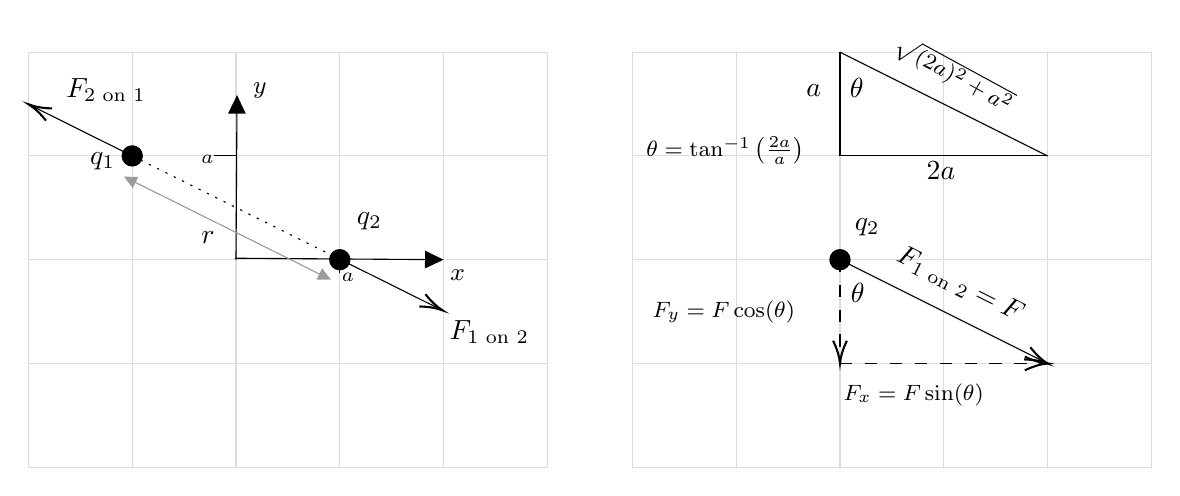
\begin{tikzpicture}[x=0.75pt,y=0.75pt,yscale=-1,xscale=1]
%uncomment if require: \path (0,244); %set diagram left start at 0, and has height of 244

%Shape: Grid [id:dp2577101908265451] 
\draw  [draw opacity=0] (313.5,12) -- (563.5,12) -- (563.5,212) -- (313.5,212) -- cycle ; \draw  [color={rgb, 255:red, 220; green, 220; blue, 220 }  ,draw opacity=1 ] (363.5,12) -- (363.5,212)(413.5,12) -- (413.5,212)(463.5,12) -- (463.5,212)(513.5,12) -- (513.5,212) ; \draw  [color={rgb, 255:red, 220; green, 220; blue, 220 }  ,draw opacity=1 ] (313.5,62) -- (563.5,62)(313.5,112) -- (563.5,112)(313.5,162) -- (563.5,162) ; \draw  [color={rgb, 255:red, 220; green, 220; blue, 220 }  ,draw opacity=1 ] (313.5,12) -- (563.5,12) -- (563.5,212) -- (313.5,212) -- cycle ;
%Shape: Grid [id:dp10244472969798668] 
\draw  [draw opacity=0] (22.5,12) -- (272.5,12) -- (272.5,212) -- (22.5,212) -- cycle ; \draw  [color={rgb, 255:red, 220; green, 220; blue, 220 }  ,draw opacity=1 ] (72.5,12) -- (72.5,212)(122.5,12) -- (122.5,212)(172.5,12) -- (172.5,212)(222.5,12) -- (222.5,212) ; \draw  [color={rgb, 255:red, 220; green, 220; blue, 220 }  ,draw opacity=1 ] (22.5,62) -- (272.5,62)(22.5,112) -- (272.5,112)(22.5,162) -- (272.5,162) ; \draw  [color={rgb, 255:red, 220; green, 220; blue, 220 }  ,draw opacity=1 ] (22.5,12) -- (272.5,12) -- (272.5,212) -- (22.5,212) -- cycle ;
%Straight Lines [id:da9013664412764533] 
\draw    (122.5,112) -- (122.98,35.71) ;
\draw [shift={(123,32.71)}, rotate = 90.36] [fill={rgb, 255:red, 0; green, 0; blue, 0 }  ][line width=0.08]  [draw opacity=0] (8.93,-4.29) -- (0,0) -- (8.93,4.29) -- cycle    ;
%Straight Lines [id:da1656851577209575] 
\draw    (122,111.29) -- (219.5,111.98) ;
\draw [shift={(222.5,112)}, rotate = 180.41] [fill={rgb, 255:red, 0; green, 0; blue, 0 }  ][line width=0.08]  [draw opacity=0] (8.93,-4.29) -- (0,0) -- (8.93,4.29) -- cycle    ;
%Shape: Circle [id:dp8533312187758539] 
\draw  [fill={rgb, 255:red, 0; green, 0; blue, 0 }  ,fill opacity=1 ] (167.63,112) .. controls (167.63,109.31) and (169.81,107.13) .. (172.5,107.13) .. controls (175.19,107.13) and (177.37,109.31) .. (177.37,112) .. controls (177.37,114.69) and (175.19,116.87) .. (172.5,116.87) .. controls (169.81,116.87) and (167.63,114.69) .. (167.63,112) -- cycle ;
%Shape: Circle [id:dp39438946029884336] 
\draw  [fill={rgb, 255:red, 0; green, 0; blue, 0 }  ,fill opacity=1 ] (67.63,62) .. controls (67.63,59.31) and (69.81,57.13) .. (72.5,57.13) .. controls (75.19,57.13) and (77.37,59.31) .. (77.37,62) .. controls (77.37,64.69) and (75.19,66.87) .. (72.5,66.87) .. controls (69.81,66.87) and (67.63,64.69) .. (67.63,62) -- cycle ;
%Straight Lines [id:da136655403531857] 
\draw  [dash pattern={on 4.5pt off 4.5pt}]  (413.5,162) -- (511.5,162) ;
\draw [shift={(513.5,162)}, rotate = 180] [color={rgb, 255:red, 0; green, 0; blue, 0 }  ][line width=0.75]    (10.93,-3.29) .. controls (6.95,-1.4) and (3.31,-0.3) .. (0,0) .. controls (3.31,0.3) and (6.95,1.4) .. (10.93,3.29)   ;
%Straight Lines [id:da2779823546963278] 
\draw  [dash pattern={on 4.5pt off 4.5pt}]  (413.5,112) -- (413.5,160) ;
\draw [shift={(413.5,162)}, rotate = 270] [color={rgb, 255:red, 0; green, 0; blue, 0 }  ][line width=0.75]    (10.93,-3.29) .. controls (6.95,-1.4) and (3.31,-0.3) .. (0,0) .. controls (3.31,0.3) and (6.95,1.4) .. (10.93,3.29)   ;
%Straight Lines [id:da33332385892304917] 
\draw    (172.25,118.64) -- (172.25,111.64) ;
%Straight Lines [id:da6065360946678762] 
\draw    (112,62) -- (122.5,62) ;
%Straight Lines [id:da542890223172384] 
\draw  [dash pattern={on 0.84pt off 2.51pt}]  (72.5,62) -- (172.25,111.64) ;
%Straight Lines [id:da6108635132526137] 
\draw [color={rgb, 255:red, 155; green, 155; blue, 155 }  ,draw opacity=1 ]   (71.19,73.34) -- (165.56,120.31) ;
\draw [shift={(168.25,121.64)}, rotate = 206.46] [fill={rgb, 255:red, 155; green, 155; blue, 155 }  ,fill opacity=1 ][line width=0.08]  [draw opacity=0] (6.25,-3) -- (0,0) -- (6.25,3) -- cycle    ;
\draw [shift={(68.5,72)}, rotate = 26.46] [fill={rgb, 255:red, 155; green, 155; blue, 155 }  ,fill opacity=1 ][line width=0.08]  [draw opacity=0] (6.25,-3) -- (0,0) -- (6.25,3) -- cycle    ;
%Straight Lines [id:da9539646965792714] 
\draw    (72.5,62) -- (24.42,38.07) ;
\draw [shift={(22.63,37.18)}, rotate = 26.46] [color={rgb, 255:red, 0; green, 0; blue, 0 }  ][line width=0.75]    (10.93,-3.29) .. controls (6.95,-1.4) and (3.31,-0.3) .. (0,0) .. controls (3.31,0.3) and (6.95,1.4) .. (10.93,3.29)   ;
%Straight Lines [id:da776994428945994] 
\draw    (413.5,112) -- (511.71,161.11) ;
\draw [shift={(513.5,162)}, rotate = 206.57] [color={rgb, 255:red, 0; green, 0; blue, 0 }  ][line width=0.75]    (10.93,-3.29) .. controls (6.95,-1.4) and (3.31,-0.3) .. (0,0) .. controls (3.31,0.3) and (6.95,1.4) .. (10.93,3.29)   ;
%Shape: Circle [id:dp8888460180413373] 
\draw  [fill={rgb, 255:red, 0; green, 0; blue, 0 }  ,fill opacity=1 ] (408.63,112) .. controls (408.63,109.31) and (410.81,107.13) .. (413.5,107.13) .. controls (416.19,107.13) and (418.37,109.31) .. (418.37,112) .. controls (418.37,114.69) and (416.19,116.87) .. (413.5,116.87) .. controls (410.81,116.87) and (408.63,114.69) .. (408.63,112) -- cycle ;
%Straight Lines [id:da7357764957591346] 
\draw    (220.33,135.57) -- (172.25,111.64) ;
\draw [shift={(222.12,136.46)}, rotate = 206.46] [color={rgb, 255:red, 0; green, 0; blue, 0 }  ][line width=0.75]    (10.93,-3.29) .. controls (6.95,-1.4) and (3.31,-0.3) .. (0,0) .. controls (3.31,0.3) and (6.95,1.4) .. (10.93,3.29)   ;
%Straight Lines [id:da027494710334365458] 
\draw    (413.5,12) -- (513.5,62) ;
%Straight Lines [id:da8224881188306552] 
\draw    (413.5,12) -- (413.5,62) ;
%Straight Lines [id:da975774904850317] 
\draw    (413.5,62) -- (513.5,62) ;

% Text Node
\draw (129.5,25.4) node [anchor=north west][inner sep=0.75pt]  [font=\small]  {$y$};
% Text Node
\draw (224.5,115.4) node [anchor=north west][inner sep=0.75pt]  [font=\small]  {$x$};
% Text Node
\draw (224.12,139.86) node [anchor=north west][inner sep=0.75pt]    {$F_{\text{1 on 2}}$};
% Text Node
\draw (179.5,88) node [anchor=north west][inner sep=0.75pt]   [align=left] {$\displaystyle q_{2}$};
% Text Node
\draw (414,170.4) node [anchor=north west][inner sep=0.75pt]  [font=\footnotesize]  {$F_{x} =F\sin (\theta )$};
% Text Node
\draw (322,130.4) node [anchor=north west][inner sep=0.75pt]  [font=\footnotesize]  {$F_{y} =F\cos (\theta )$};
% Text Node
\draw (172.25,117.04) node [anchor=north west][inner sep=0.75pt]  [font=\scriptsize]  {$a$};
% Text Node
\draw (104.5,60.4) node [anchor=north west][inner sep=0.75pt]  [font=\scriptsize]  {$a$};
% Text Node
\draw (104.5,97) node [anchor=north west][inner sep=0.75pt]   [align=left] {$\displaystyle r$};
% Text Node
\draw (39.5,23.4) node [anchor=north west][inner sep=0.75pt]    {$F_{\text{2 on 1}}$};
% Text Node
\draw (51,59) node [anchor=north west][inner sep=0.75pt]   [align=left] {$\displaystyle q_{1}$};
% Text Node
\draw (419.37,91) node [anchor=north west][inner sep=0.75pt]   [align=left] {$\displaystyle q_{2}$};
% Text Node
\draw (443.76,102.48) node [anchor=north west][inner sep=0.75pt]  [rotate=-26.6]  {$F_{\text{1 on 2}} =F$};
% Text Node
\draw (454,63.4) node [anchor=north west][inner sep=0.75pt]    {$2a$};
% Text Node
\draw (396,26.4) node [anchor=north west][inner sep=0.75pt]    {$a$};
% Text Node
\draw (417,23.4) node [anchor=north west][inner sep=0.75pt]    {$\theta $};
% Text Node
\draw (417.5,122.27) node [anchor=north west][inner sep=0.75pt]    {$\theta $};
% Text Node
\draw (319,51.4) node [anchor=north west][inner sep=0.75pt]  [font=\footnotesize]  {$\theta =\tan^{-1}\left(\frac{2a}{a}\right)$};
% Text Node
\draw (443.42,0.48) node [anchor=north west][inner sep=0.75pt]  [font=\footnotesize,rotate=-28.54]  {$\sqrt{( 2a)^{2} +a^{2}}$};


\end{tikzpicture}


    \begin{enumerate}

      \item $\ds F_{1\mbox{ on } 2}=k\frac{|q_1q_2|}{r^2}=\frac{k|qq|}{(\sqrt{(2a)^2+a^2})^2}=\frac{kq^2}{5a^2}$

      \item $\bfvec{F}_{1\mbox{ on } 2} = F_{1\mbox{ on } 2}(\sin \theta \ihat - \cos \theta\jhat)$, where $\theta=\tan^{-1}(2) = 63.4^\circ$.

                Alternatively, from the diagram on the right, $\sin\theta = 2a/\sqrt{5}a$ and $\cos\theta = 1a/\sqrt{5}a$, so 
                $\ds\bfvec{F}_{1\mbox{ on } 2} = F_{1\mbox{ on } 2}\left(\frac{2}{\sqrt{5}}\ihat - \frac{1}{\sqrt{5}}\jhat\right)$.

    \end{enumerate}
\else



\tikzset{every picture/.style={line width=0.75pt}} %set default line width to 0.75pt        


\begin{tikzpicture}[x=0.75pt,y=0.75pt,yscale=-1,xscale=1]
%uncomment if require: \path (0,208); %set diagram left start at 0, and has height of 208

%Shape: Grid [id:dp33505564538856114] 
\draw  [draw opacity=0] (2,2) -- (552,2) -- (552,202) -- (2,202) -- cycle ; \draw  [color={rgb, 255:red, 220; green, 220; blue, 220 }  ,draw opacity=1 ] (52,2) -- (52,202)(102,2) -- (102,202)(152,2) -- (152,202)(202,2) -- (202,202)(252,2) -- (252,202)(302,2) -- (302,202)(352,2) -- (352,202)(402,2) -- (402,202)(452,2) -- (452,202)(502,2) -- (502,202) ; \draw  [color={rgb, 255:red, 220; green, 220; blue, 220 }  ,draw opacity=1 ] (2,52) -- (552,52)(2,102) -- (552,102)(2,152) -- (552,152) ; \draw  [color={rgb, 255:red, 220; green, 220; blue, 220 }  ,draw opacity=1 ] (2,2) -- (552,2) -- (552,202) -- (2,202) -- cycle ;




\end{tikzpicture}

\fi

\section{Problem III}

Answer questions 1.--3. of Problem I for charge $q_1$ is at $(x,y)=(-a,0)$ and charge $q_2$ is at $(0, 3a)$. Charge $q_1$ has a charge of $-q$. Charge $q_2$ has a charge of $+q$.

\ifsolutions
{\bf Solution}


\tikzset{every picture/.style={line width=0.75pt}} %set default line width to 0.75pt        

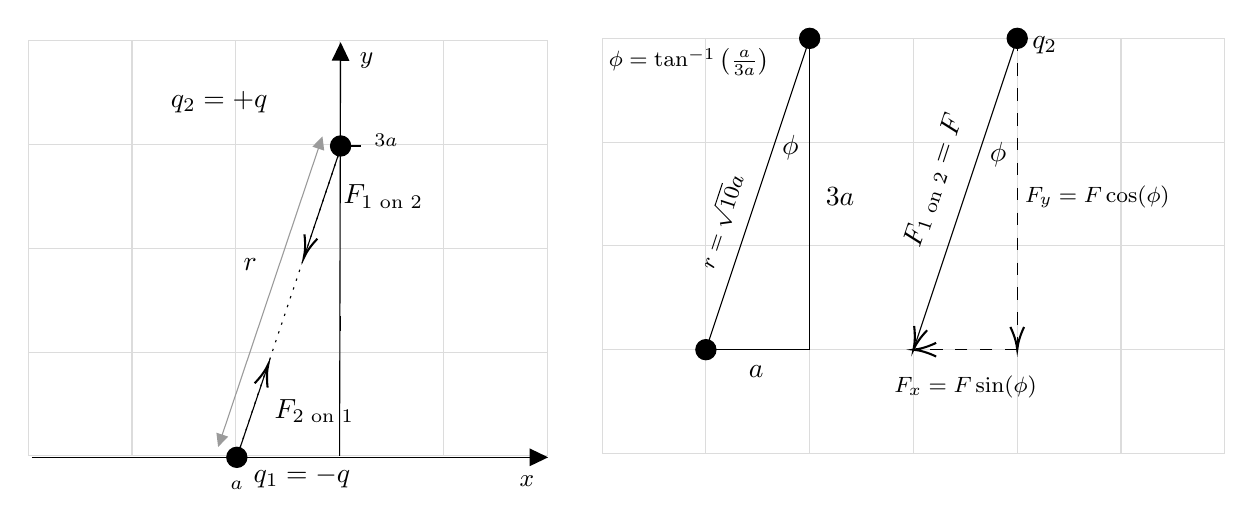
\begin{tikzpicture}[x=0.75pt,y=0.75pt,yscale=-1,xscale=1]
%uncomment if require: \path (0,244); %set diagram left start at 0, and has height of 244

%Shape: Grid [id:dp06901313689897681] 
\draw  [draw opacity=0] (22,5.95) -- (272,5.95) -- (272,205.95) -- (22,205.95) -- cycle ; \draw  [color={rgb, 255:red, 220; green, 220; blue, 220 }  ,draw opacity=1 ] (72,5.95) -- (72,205.95)(122,5.95) -- (122,205.95)(172,5.95) -- (172,205.95)(222,5.95) -- (222,205.95) ; \draw  [color={rgb, 255:red, 220; green, 220; blue, 220 }  ,draw opacity=1 ] (22,55.95) -- (272,55.95)(22,105.95) -- (272,105.95)(22,155.95) -- (272,155.95) ; \draw  [color={rgb, 255:red, 220; green, 220; blue, 220 }  ,draw opacity=1 ] (22,5.95) -- (272,5.95) -- (272,205.95) -- (22,205.95) -- cycle ;
%Shape: Grid [id:dp6986252894167704] 
\draw  [draw opacity=0] (298.5,4.81) -- (598.5,4.81) -- (598.5,204.81) -- (298.5,204.81) -- cycle ; \draw  [color={rgb, 255:red, 220; green, 220; blue, 220 }  ,draw opacity=1 ] (348.5,4.81) -- (348.5,204.81)(398.5,4.81) -- (398.5,204.81)(448.5,4.81) -- (448.5,204.81)(498.5,4.81) -- (498.5,204.81)(548.5,4.81) -- (548.5,204.81) ; \draw  [color={rgb, 255:red, 220; green, 220; blue, 220 }  ,draw opacity=1 ] (298.5,54.81) -- (598.5,54.81)(298.5,104.81) -- (598.5,104.81)(298.5,154.81) -- (598.5,154.81) ; \draw  [color={rgb, 255:red, 220; green, 220; blue, 220 }  ,draw opacity=1 ] (298.5,4.81) -- (598.5,4.81) -- (598.5,204.81) -- (298.5,204.81) -- cycle ;
%Straight Lines [id:da10801395440171135] 
\draw    (172,205.95) -- (172.49,9.67) ;
\draw [shift={(172.5,6.67)}, rotate = 90.14] [fill={rgb, 255:red, 0; green, 0; blue, 0 }  ][line width=0.08]  [draw opacity=0] (8.93,-4.29) -- (0,0) -- (8.93,4.29) -- cycle    ;
%Straight Lines [id:da6569767004405282] 
\draw    (23.72,206.67) -- (269.5,206.67) ;
\draw [shift={(272.5,206.67)}, rotate = 180] [fill={rgb, 255:red, 0; green, 0; blue, 0 }  ][line width=0.08]  [draw opacity=0] (8.93,-4.29) -- (0,0) -- (8.93,4.29) -- cycle    ;
%Shape: Circle [id:dp9980789777094827] 
\draw  [fill={rgb, 255:red, 0; green, 0; blue, 0 }  ,fill opacity=1 ] (117.63,206.67) .. controls (117.63,203.97) and (119.81,201.79) .. (122.5,201.79) .. controls (125.19,201.79) and (127.37,203.97) .. (127.37,206.67) .. controls (127.37,209.36) and (125.19,211.54) .. (122.5,211.54) .. controls (119.81,211.54) and (117.63,209.36) .. (117.63,206.67) -- cycle ;
%Shape: Circle [id:dp38639083005377794] 
\draw  [fill={rgb, 255:red, 0; green, 0; blue, 0 }  ,fill opacity=1 ] (167.63,56.67) .. controls (167.63,53.97) and (169.81,51.79) .. (172.5,51.79) .. controls (175.19,51.79) and (177.37,53.97) .. (177.37,56.67) .. controls (177.37,59.36) and (175.19,61.54) .. (172.5,61.54) .. controls (169.81,61.54) and (167.63,59.36) .. (167.63,56.67) -- cycle ;
%Straight Lines [id:da8264911542578002] 
\draw  [dash pattern={on 4.5pt off 4.5pt}]  (498.5,154.81) -- (450.5,154.81) ;
\draw [shift={(448.5,154.81)}, rotate = 360] [color={rgb, 255:red, 0; green, 0; blue, 0 }  ][line width=0.75]    (10.93,-3.29) .. controls (6.95,-1.4) and (3.31,-0.3) .. (0,0) .. controls (3.31,0.3) and (6.95,1.4) .. (10.93,3.29)   ;
%Straight Lines [id:da22948629211472427] 
\draw  [dash pattern={on 4.5pt off 4.5pt}]  (498.5,4.81) -- (498.5,152.81) ;
\draw [shift={(498.5,154.81)}, rotate = 270] [color={rgb, 255:red, 0; green, 0; blue, 0 }  ][line width=0.75]    (10.93,-3.29) .. controls (6.95,-1.4) and (3.31,-0.3) .. (0,0) .. controls (3.31,0.3) and (6.95,1.4) .. (10.93,3.29)   ;
%Straight Lines [id:da30634899776468916] 
\draw    (172.25,145.64) -- (172.25,138.64) ;
%Straight Lines [id:da6777094424125605] 
\draw    (172,56.67) -- (182.5,56.67) ;
%Straight Lines [id:da5535038032697024] 
\draw  [dash pattern={on 0.84pt off 2.51pt}]  (172.75,57.02) -- (122.5,206.67) ;
%Straight Lines [id:da11385133765268529] 
\draw [color={rgb, 255:red, 155; green, 155; blue, 155 }  ,draw opacity=1 ]   (114.45,198.82) -- (162.8,54.87) ;
\draw [shift={(163.75,52.02)}, rotate = 108.56] [fill={rgb, 255:red, 155; green, 155; blue, 155 }  ,fill opacity=1 ][line width=0.08]  [draw opacity=0] (6.25,-3) -- (0,0) -- (6.25,3) -- cycle    ;
\draw [shift={(113.5,201.67)}, rotate = 288.56] [fill={rgb, 255:red, 155; green, 155; blue, 155 }  ,fill opacity=1 ][line width=0.08]  [draw opacity=0] (6.25,-3) -- (0,0) -- (6.25,3) -- cycle    ;
%Straight Lines [id:da03037209404476293] 
\draw    (172.75,57.02) -- (155.36,108.77) ;
\draw [shift={(154.72,110.67)}, rotate = 288.58] [color={rgb, 255:red, 0; green, 0; blue, 0 }  ][line width=0.75]    (10.93,-3.29) .. controls (6.95,-1.4) and (3.31,-0.3) .. (0,0) .. controls (3.31,0.3) and (6.95,1.4) .. (10.93,3.29)   ;
%Straight Lines [id:da20421055105636987] 
\draw    (137.08,163.56) -- (122.5,206.67) ;
\draw [shift={(137.72,161.67)}, rotate = 108.69] [color={rgb, 255:red, 0; green, 0; blue, 0 }  ][line width=0.75]    (10.93,-3.29) .. controls (6.95,-1.4) and (3.31,-0.3) .. (0,0) .. controls (3.31,0.3) and (6.95,1.4) .. (10.93,3.29)   ;
%Straight Lines [id:da7663366897025317] 
\draw    (398.5,4.81) -- (348.5,154.81) ;
%Straight Lines [id:da7723714363889567] 
\draw    (398.5,4.81) -- (398.5,154.81) ;
%Straight Lines [id:da13067723851525392] 
\draw    (348.5,154.81) -- (398.5,154.81) ;
%Straight Lines [id:da7342958637009416] 
\draw    (498.5,4.81) -- (449.13,152.91) ;
\draw [shift={(448.5,154.81)}, rotate = 288.43] [color={rgb, 255:red, 0; green, 0; blue, 0 }  ][line width=0.75]    (10.93,-3.29) .. controls (6.95,-1.4) and (3.31,-0.3) .. (0,0) .. controls (3.31,0.3) and (6.95,1.4) .. (10.93,3.29)   ;
%Shape: Circle [id:dp6424795947790023] 
\draw  [fill={rgb, 255:red, 0; green, 0; blue, 0 }  ,fill opacity=1 ] (493.63,4.81) .. controls (493.63,2.12) and (495.81,-0.07) .. (498.5,-0.07) .. controls (501.19,-0.07) and (503.37,2.12) .. (503.37,4.81) .. controls (503.37,7.5) and (501.19,9.68) .. (498.5,9.68) .. controls (495.81,9.68) and (493.63,7.5) .. (493.63,4.81) -- cycle ;
%Shape: Circle [id:dp05793815285939008] 
\draw  [fill={rgb, 255:red, 0; green, 0; blue, 0 }  ,fill opacity=1 ] (343.63,154.81) .. controls (343.63,152.12) and (345.81,149.93) .. (348.5,149.93) .. controls (351.19,149.93) and (353.37,152.12) .. (353.37,154.81) .. controls (353.37,157.5) and (351.19,159.68) .. (348.5,159.68) .. controls (345.81,159.68) and (343.63,157.5) .. (343.63,154.81) -- cycle ;
%Shape: Circle [id:dp06509808379524396] 
\draw  [fill={rgb, 255:red, 0; green, 0; blue, 0 }  ,fill opacity=1 ] (393.63,4.81) .. controls (393.63,2.12) and (395.81,-0.07) .. (398.5,-0.07) .. controls (401.19,-0.07) and (403.37,2.12) .. (403.37,4.81) .. controls (403.37,7.5) and (401.19,9.68) .. (398.5,9.68) .. controls (395.81,9.68) and (393.63,7.5) .. (393.63,4.81) -- cycle ;

% Text Node
\draw (180.5,10.4) node [anchor=north west][inner sep=0.75pt]  [font=\small]  {$y$};
% Text Node
\draw (257.5,214.4) node [anchor=north west][inner sep=0.75pt]  [font=\small]  {$x$};
% Text Node
\draw (172.73,74.24) node [anchor=north west][inner sep=0.75pt]    {$F_{\text{1 on 2}}$};
% Text Node
\draw (89.5,29) node [anchor=north west][inner sep=0.75pt]   [align=left] {$\displaystyle q_{2} =+q$};
% Text Node
\draw (438,166.4) node [anchor=north west][inner sep=0.75pt]  [font=\footnotesize]  {$F_{x} =F\sin (\phi )$};
% Text Node
\draw (501,74.4) node [anchor=north west][inner sep=0.75pt]  [font=\footnotesize]  {$F_{y} =F\cos (\phi )$};
% Text Node
\draw (118.25,217.04) node [anchor=north west][inner sep=0.75pt]  [font=\scriptsize]  {$a$};
% Text Node
\draw (187.5,49.4) node [anchor=north west][inner sep=0.75pt]  [font=\scriptsize]  {$3a$};
% Text Node
\draw (124.5,109.67) node [anchor=north west][inner sep=0.75pt]   [align=left] {$\displaystyle r$};
% Text Node
\draw (139.5,177.4) node [anchor=north west][inner sep=0.75pt]    {$F_{\text{2 on 1}}$};
% Text Node
\draw (129.37,209.67) node [anchor=north west][inner sep=0.75pt]   [align=left] {$\displaystyle q_{1} =-q$};
% Text Node
\draw (441.28,103.8) node [anchor=north west][inner sep=0.75pt]  [rotate=-288.2]  {$F_{\text{1 on 2}} =F$};
% Text Node
\draw (405,75.4) node [anchor=north west][inner sep=0.75pt]    {$3a$};
% Text Node
\draw (368,161.4) node [anchor=north west][inner sep=0.75pt]    {$a$};
% Text Node
\draw (384,50.4) node [anchor=north west][inner sep=0.75pt]    {$\phi $};
% Text Node
\draw (300.5,8.21) node [anchor=north west][inner sep=0.75pt]  [font=\footnotesize]  {$\phi =\tan^{-1}\left(\frac{a}{3a}\right)$};
% Text Node
\draw (341.25,114.37) node [anchor=north west][inner sep=0.75pt]  [font=\footnotesize,rotate=-288.25]  {$r=\sqrt{10} a$};
% Text Node
\draw (484,53.4) node [anchor=north west][inner sep=0.75pt]    {$\phi $};
% Text Node
\draw (504.5,2.81) node [anchor=north west][inner sep=0.75pt]   [align=left] {$\displaystyle q_{2}$};


\end{tikzpicture}


    \begin{enumerate}

      \item $r=\sqrt{a^2+(3a)^2}$, $F=k|q(-q)|/r^2=kq^2/10a^2$

      \item The angle $\theta$ shown in the diagram is $\theta=\tan^{-1}(1/3)=18.4^\circ$, so the angle with respect to the $+x$--axis is $270-18.4=251.6^\circ$

      \item $\bfvec{F}=F\sin251.6^\circ\ihat - F\cos251.6^\circ\jhat$

            or

            $\bfvec{F}=-F\sin 18.4^\circ\ihat - F\cos18.4^\circ\jhat$

            Alternatively, from the diagram,

            $\sin\theta = a/\sqrt{10}a$ and $\cos\theta = 3a/\sqrt{10}a$, so

            $\ds\bfvec{F}_{1\mbox{ on } 2} = F\left(-\frac{1}{\sqrt{10}}\ihat - \frac{3}{\sqrt{10}}\jhat\right)$

    \end{enumerate}
\else



\tikzset{every picture/.style={line width=0.75pt}} %set default line width to 0.75pt        


\begin{tikzpicture}[x=0.75pt,y=0.75pt,yscale=-1,xscale=1]
%uncomment if require: \path (0,208); %set diagram left start at 0, and has height of 208

%Shape: Grid [id:dp33505564538856114] 
\draw  [draw opacity=0] (2,2) -- (552,2) -- (552,202) -- (2,202) -- cycle ; \draw  [color={rgb, 255:red, 220; green, 220; blue, 220 }  ,draw opacity=1 ] (52,2) -- (52,202)(102,2) -- (102,202)(152,2) -- (152,202)(202,2) -- (202,202)(252,2) -- (252,202)(302,2) -- (302,202)(352,2) -- (352,202)(402,2) -- (402,202)(452,2) -- (452,202)(502,2) -- (502,202) ; \draw  [color={rgb, 255:red, 220; green, 220; blue, 220 }  ,draw opacity=1 ] (2,52) -- (552,52)(2,102) -- (552,102)(2,152) -- (552,152) ; \draw  [color={rgb, 255:red, 220; green, 220; blue, 220 }  ,draw opacity=1 ] (2,2) -- (552,2) -- (552,202) -- (2,202) -- cycle ;




\end{tikzpicture}

\fi

\section{Problem IV}

Charge $q_1$ is at $(x,y)=(x_1,y_1)$ and charge $q_2$ is at $(x_2, y_2)$. Find the magnitude of the force of $q_1$ on $q_2$.

\ifsolutions
{\bf Solution}: $F=k|q_1q_2|/\left((x_2-x_1)^2 + (y_2-y_1)^2\right)$. Make sure that you can justify this with a diagram. Check to see if you can use this formula to find the magnitudes for the previous problems.
\fi

\end{document}